\documentclass[11pt]{amsart}
\input{glyphtounicode}
\pdfgentounicode=1
\usepackage[T1]{fontenc}
\usepackage[utf8]{inputenc}
\usepackage{amsmath,amssymb}
\usepackage{array,booktabs,tabularx}
\usepackage{graphicx}
\usepackage{xcolor}
\usepackage{geometry}
\usepackage{enumitem}
\usepackage{hyperref}
\geometry{margin=1in}
\setlength{\emergencystretch}{3em}
\graphicspath{{../tree_stability_v4/figures/}}
\hypersetup{colorlinks=true,linkcolor=blue!45!black,citecolor=blue!45!black,urlcolor=blue!45!black,
  pdftitle={SEION Math Core v5: Software, Evidence, and Reproducibility},
  pdfauthor={Eliuth Chavero Jasso},
  pdfsubject={Research software and artifact protocol for projected multilinear tree and graph certificates},
  pdfkeywords={research software, reproducibility, artifact governance, multilinear graphs}}
\title[SEION Math Core v5 software]{SEION Math Core v5: Software, Evidence, and Reproducibility for Projected Multilinear Graphs}
\author{Eliuth Chavero Jasso}
\address{Independent Researcher, Apizaco, Tlaxcala, Mexico}
\thanks{Software and reproducibility companion. This paper does not constitute theorem approval, novelty approval, or release authorization.}
\date{8 August 2026 -- v5 research companion}

\begin{document}
\begin{abstract}
This companion documents the repository architecture, evidence contracts, test gates, paper-generation workflow, and governance state for the finite projected multilinear tree and graph program. The package separates executable behavior, mathematical claims, numerical artifacts, experiments, durable memory, and publication outputs. The v5 research layer adds an exact independent-law $k=2$ sharpness construction, $k=3$ lower witnesses, source-polynomial DAG propagation, signed-expression certificates, validated finite norm enclosures, and approximate-law budgets. The latest focused suite contains 85 passing tests; governance passes structurally with known historical warnings. The package remains fail-closed for theorem novelty, independent human review, and global sharpness.\end{abstract}
\subjclass[2020]{68N30, 65Y05, 65G50, 15A69}
\keywords{research software, reproducibility, artifact contract, projected multilinear graph, governance}
\maketitle

\section{Repository and evidence separation}

The repository follows a source-of-truth policy. Executable behavior lives in
\texttt{src/} and tests. Mathematical status lives in theorem and claim
registries, proof dossiers, and counterexample records. Executed numerical
facts live in manifests, metrics, certificates, and artifact hashes.
Experiments live in registered matrices. Durable project state lives in
\texttt{.ai/}. Generated paper tables and figures are derived outputs with
provenance, never manual authorities.

This separation prevents a passing software test, a polished PDF, or a
generated metric from silently becoming a universal mathematical statement.
The governance contract distinguishes declared, observed, verified, and
approved authority levels; human approval remains a separate gate.

\section{Finite-core lineage}

The finite v4 mathematical/software core is frozen at scientific commit
\texttt{1f4984ec}; the complete SHA is preserved in the package manifest. The
v5 theorem track then records the following immutable checkpoints:

\begin{center}
\small
\begin{tabularx}{.97\textwidth}{@{}l l X@{}}
\toprule
checkpoint & role & scope\\
\midrule
\texttt{10078f4} & V5 k=2 construction & independent-law saturation and equality audit\\
\texttt{773fa9c} & V5 freeze metadata & scientific baseline and ledger binding\\
\texttt{5e8384a} & V5-A construction & independent-law k=3 chain/branch lower witnesses\\
\texttt{997e745} & V5-A registry & lower-bound and conjecture status registration\\
\bottomrule
\end{tabularx}
\end{center}

The operational branch is \texttt{campaign/gate13-closeout}. Gate 13.5, Gate
14, KGR, and historical run trees are preserved and are not part of the v5
paper-generation change.

\section{Source architecture}

The research implementation is intentionally split by generation:

\begin{center}
\footnotesize
\begin{tabularx}{.97\textwidth}{@{}lX@{}}
\toprule
path & responsibility\\
\midrule
\texttt{src/seion\_core/research\_v3} & typed trees, exact/projected evaluation, nodewise certificates, enumeration\\
\texttt{src/seion\_core/research\_v4} & scalar DAG, source-aware, higher-order, signed, norm, and approximate-law layers\\
\texttt{src/seion\_core/research\_v5} & theorem-level k=2 sharpness, equality audit, and k=3 independent-law witnesses\\
\texttt{research/projected\_trees\_v4} & finite-core proof dossiers and registries\\
\texttt{research/projected\_trees\_v5} & V5 truth ledger, manuscript consolidation, formal targets, and novelty matrix\\
\texttt{claims/} & theorem, claim, counterexample, and novelty authority registries\\
\texttt{.ai/} & durable memory, tasks, decisions, blockers, evidence ledger, and handoff history\\
\bottomrule
\end{tabularx}
\end{center}

\section{Verification gates}

The focused v5 validation command is:
\begin{verbatim}
python -m pytest tests/research_v3 tests/research_v4 \\
  tests/research_v5_test_k2_sharpness.py \\
  tests/research_v5_test_equality_conditions.py \\
  tests/research_v5_test_k3_independent_candidates.py -q
\end{verbatim}
It currently reports 85 passing tests. These include exact subset expansion,
projected-root geometry, scalar and source-aware DAG certificates, repeated
source multi-indices, signed cancellation, norm metadata, approximate-law
budgets, k=2 exact saturation, equality compatibility, and k=3 lower-witness
checks.

\section{Artifact and provenance contract}

Every registered run records identity, resolved configuration, command,
environment, hardware, mathematical-object hashes, input hashes, metrics,
certificates, logs, and artifact hashes. Historical runs remain immutable;
deduplication creates a derived unique index rather than deleting records.
The latest structural audit reports 150 historical runs, 9 unique scientific
instances, 8 duplicate groups, 0 missing artifacts, and complete contracts for
all 150 records. The duplicate warning is a governance issue, not a reason to
reinterpret historical runs as independent evidence.

\section{Paper-generation workflow}

The v5 paper sources are under
\texttt{papers/projected\_graphs\_v5}. They reuse registered v4 vector figures
and bibliography while adding only claims supported by the V5 truth ledger.
The build script compiles each source with \texttt{latexmk}, writes final PDFs
to \texttt{output/pdf/}, runs \texttt{pdfinfo} and text extraction checks, and
renders pages with Poppler for visual inspection. Generated auxiliary files
remain in the intermediate build area and are not treated as scientific
artifacts.

\begin{figure}[p]
\centering
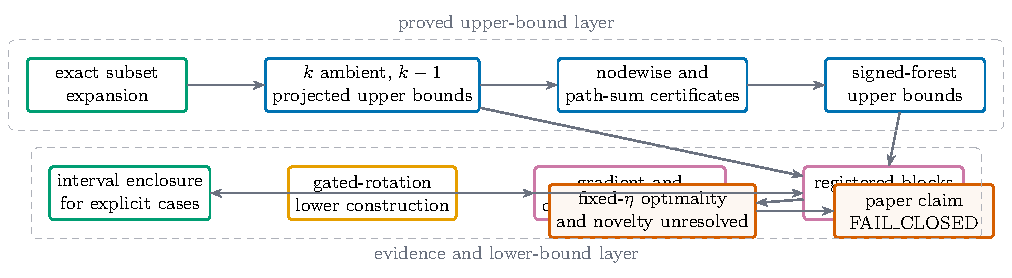
\includegraphics[width=.94\textwidth]{fig18_claim_evidence_dag}
\caption{The evidence DAG separates proof, upper certificate, lower construction, empirical search, and release authorization.}
\end{figure}

\section{Governance and limitations}

The current governance result is non-strict PASS/YELLOW. Required artifacts
are present; warnings remain for duplicate historical runs and the paper
quality rubric. The strict research gate remains fail-closed because
theorem-level novelty, independent human review, repeated-law sharpness,
global $k=3$ sharpness, universal dimension/rank reduction, and global
multilinear norm optimality are unresolved.

A compiled PDF is therefore a reproducible research artifact, not publication
approval. No test-set or KGR claim is changed by this package.

\section{Reproduction checklist}

\begin{enumerate}[leftmargin=*]
\item Read \texttt{AGENTS.md}, the memory manifest, current state, tasks, and blockers.
\item Inspect the relevant theorem and truth ledgers before changing a claim.
\item Run the focused pytest command and JSON validation.
\item Run governance audit and run deduplication.
\item Compile the three papers and render every final PDF page.
\item Record command, environment, branch, commit, changed files, and limitations in postflight.
\end{enumerate}

\section{Conclusion}

The software package is experiment-ready and paper-build-ready, but not
release-approved. Its primary value is that every mathematical statement,
construction, test, artifact, and limitation has a durable location and a
reproducible command path.

\nocite{SIAMReproducibility2026,Higham2002,MooreKearfottCloud2009}
\bibliographystyle{amsplain}
\bibliography{references}
\end{document}
